\documentclass[12pt,a4paper,twoside]{article}
\newcommand{\studentname}{Giuseppe Nobile 1000001179}
\title{Weighted Feedback Vertex Set Problem using HGA algorithm}

\newcommand{\tutor}{Mario Francesco Pavone, Vincenzo Cutello}

\newcommand{\reportdate}{03/03/2025}
\newcommand{\department}{D.M.I. Informatica LM-18 A.A. 2024/2025}
\usepackage{float}     % per l'opzione [H]
\usepackage[a4paper, margin=1in]{geometry}
\usepackage[a4paper,left=32mm,right=32mm,bottom=32mm,top=32mm]{geometry}
\usepackage{listings}
\usepackage{color}
\usepackage{fancyhdr}
\usepackage{subfigure}
\usepackage{graphicx}
\usepackage{booktabs}
\usepackage[british]{babel}
\usepackage[square,comma,numbers,sort&compress]{natbib}
\usepackage{csvsimple}
\usepackage{graphicx}
\usepackage{pgfplotstable,filecontents}
\usepackage{gensymb}
\usepackage{array}
\usepackage{tabu}
\usepackage{multirow}
\usepackage{url}
\usepackage{hyperref}
\usepackage{amsmath}
\documentclass{article}
\usepackage{amssymb}
\usepackage{algorithm}
\usepackage{algorithmicx}
\usepackage{algpseudocode}
\urlstyle{same}
\usepackage{cleveref}
\pgfplotsset{compat=1.9}
\definecolor{bg}{RGB}{240,240,240}
\usepackage[utf8]{inputenc}
\usepackage[T1]{fontenc}
\usepackage{imakeidx}
\makeindex[columns=1, title=Indice]
\usepackage{enumitem}
\usepackage{graphicx}   



\begin{document}
\author{\studentname ~ \\ \\ Professori: \tutor.\\
\\
Dipartimento: \department}

\date{Data documento: \reportdate.}

\renewcommand\abstractname{Summary}

\pagestyle{fancy}
\fancyhead{}
\fancyhead[C]{\studentname~}
\fancyfoot{}
\fancyfoot[C]{\thepage}
\renewcommand{\headrulewidth}{0pt}
\renewcommand{\footrulewidth}{0pt}

\renewcommand\bibname{Riferimenti}
\renewcommand*\contentsname{Indice}
\renewcommand{\figurename}{Fig.}
\renewcommand{\tablename}{Tab.}

\begin{figure}[h!]
    \centering
    \maketitle
\end{figure}

\tableofcontents
\clearpage

\section{Weighted Feedback Vertex Set Problem}
Il problema del \emph{Feedback Vertex Set} (FVS) rappresenta un interessante problema di ottimizzazione combinatoria che consiste nel trovare un sottoinsieme di vertici tale che, rimuovendoli da un grafo, si ottenga un grafo aciclico. La risoluzione del problema FVS gioca un ruolo fondamentale nei sistemi operativi e nel calcolo parallelo, poiché, in un \emph{wait-for graph}, ogni ciclo diretto corrisponde ad una situazione di deadlock. In questo contesto, il feedback vertex set consente di individuare il numero minimo di processi bloccati che devono essere abortiti per eliminare il deadlock. Inoltre, il problema FVS trova applicazione anche nella teoria della complessità, dove alcuni problemi difficili sui grafi possono essere risolti in tempo polinomiale se il numero dei vertici in un FVS è limitato. Altre applicazioni pratiche includono la verifica dei programmi, la sicurezza informatica e lo studio dei monopoli in sistemi distribuiti sincroni.

\bigskip

\subsection{Definizione formale del WFVS}
Sia \( G = (V, E) \) un grafo non orientato. Un \emph{feedback vertex set} di \( G \) è un sottoinsieme \( S \subseteq V \) di vertici tale che, rimuovendo \( S \) e tutti gli archi incidenti ai vertici di \( S \), il grafo risultante \( G[V \setminus S] \) sia aciclico. Se inoltre è definita una funzione di peso \( w : V \rightarrow \mathbb{R}^+ \) che assegna ad ogni vertice \( v \in V \) un valore positivo, il peso del feedback vertex set \( S \) è dato da
\[
\sum_{v \in S} w(v).
\]
Il problema del \emph{Weighted Feedback Vertex Set} consiste nel trovare un feedback vertex set \( S \) di peso minimo, ovvero:
\[
\text{minimizzare } \sum_{v \in S} w(v).
\]
\section{HGA algorithm}
L'algoritmo HGA (Hybrid Genetic Algorithm) rappresenta un approccio metaeuristico ibrido che integra le strategie degli algoritmi genetici classici con tecniche di ottimizzazione locale, al fine di migliorare la capacità di esplorazione e sfruttamento dello spazio delle soluzioni in problemi complessi e spesso NP-hard. In maniera formale, l'HGA inizia con la generazione di una popolazione iniziale \( P_0 \) di soluzioni candidate, ognuna rappresentata da un cromosoma che codifica una possibile configurazione del problema. Ad ogni iterazione, o generazione, viene eseguita una procedura di selezione basata sul valore della funzione obiettivo \( f \), seguita dall'applicazione degli operatori genetici di crossover e mutazione, che consentono la creazione di nuove soluzioni sfruttando le informazioni derivanti da quelle esistenti. A differenza degli algoritmi genetici tradizionali, l'HGA incorpora una fase di \emph{ricerca locale} che, applicata ai candidati prodotti, raffina ulteriormente le soluzioni migliorandone la qualità mediante tecniche di ottimizzazione deterministica o euristica. Formalmente, data una soluzione \( x \) generata tramite gli operatori genetici, viene eseguita una procedura di \emph{local search} per trovare una soluzione \( x' \) tale che
\[
f(x') \leq f(x)
\]
(oppure \( f(x') \geq f(x) \) nel caso di massimizzazione), garantendo così un'ulteriore discesa lungo la funzione obiettivo. Il ciclo iterativo tra evoluzione genetica e ottimizzazione locale prosegue fino al raggiungimento di un criterio di arresto predeterminato, come un numero massimo di iterazioni o la convergenza della popolazione. Questa combinazione sinergica permette all'HGA di bilanciare efficacemente l’esplorazione globale dello spazio delle soluzioni con un’accurata intensificazione della ricerca nelle regioni promettenti, rendendolo particolarmente adatto per affrontare problemi di elevata complessità computazionale.
\subsection{Definizione formale}
Sia dato un problema di ottimizzazione definito sullo spazio delle soluzioni \(\mathcal{S}\) mediante la funzione obiettivo
\[
f:\mathcal{S}\to\mathbb{R},
\]
dove l'obiettivo è minimizzare \(f\). L'algoritmo \emph{Hybrid Genetic Algorithm} (HGA) costruisce una successione di popolazioni \(\{P_t\}_{t=0}^T\) di dimensione \(N\), ovvero:
\[
P_t \subseteq \mathcal{S} \quad \text{con} \quad |P_t| = N,\quad t=0,1,\dots,T.
\]
La procedura iterativa dell'HGA si articola tramite i seguenti operatori:

\begin{enumerate}
    \item \textbf{Selezione:} Definiamo l'operatore di selezione
    \[
    \operatorname{Select}: \mathcal{P}(\mathcal{S}) \to \mathcal{S},
    \]
    che, applicato alla popolazione corrente \(P_t\), genera un mating pool \(M_t \subseteq P_t\) in cui la probabilità di selezione di un individuo \(x\) è inversamente proporzionale a \(f(x)\) (nel caso di minimizzazione).

    \item \textbf{Crossover:} L'operatore di crossover
    \[
    \operatorname{Cross}: \mathcal{S} \times \mathcal{S} \to \mathcal{S},
    \]
    combina coppie di individui \((x_i, x_j) \in M_t \times M_t\) per produrre nuovi discendenti.

    \item \textbf{Mutazione:} L'operatore di mutazione
    \[
    \operatorname{Mutate}: \mathcal{S} \to \mathcal{S},
    \]
    introduce variazioni casuali nei discendenti, garantendo la diversità genetica all'interno della popolazione.

    \item \textbf{Ricerca Locale:} L'operatore di ricerca locale
    \[
    \operatorname{LS}: \mathcal{S} \to \mathcal{S},
    \]
    applica una procedura di ottimizzazione su un intorno della soluzione \(x\), ottenendo una soluzione migliorata \(x' = \operatorname{LS}(x)\) tale che
    \[
    f(x') \leq f(x).
    \]

    \item \textbf{Sostituzione:} Infine, una strategia di sostituzione \(\operatorname{Replace}\) aggiorna la popolazione, combinando i discendenti (ottimizzati localmente) con alcuni individui della popolazione corrente, per formare la nuova popolazione \(P_{t+1}\).
\end{enumerate}

La procedura iterativa dell'HGA si può formalizzare come:
\[
P_{t+1} = \operatorname{Replace}\Bigl(P_t,\ \operatorname{LS}\Bigl(\operatorname{Mutate}\bigl(\operatorname{Cross}(\operatorname{Select}(P_t))\bigr)\Bigr)\Bigr),
\]
con \(t = 0, 1, \dots, T-1\), e con una condizione di terminazione definita (ad esempio, un numero massimo di iterazioni \(T\) oppure il raggiungimento di una soglia di miglioramento).

Al termine dell'esecuzione, l'algoritmo restituisce il miglior individuo:
\[
x^* = \arg\min_{x \in P_T} f(x),
\]
che rappresenta l'approssimazione ottimale (o una buona soluzione) del problema di ottimizzazione.

\bigskip
Questa definizione formale evidenzia come l'integrazione di operatori genetici tradizionali con tecniche di ricerca locale permetta all'HGA di bilanciare in maniera efficace l'esplorazione globale e l'intensificazione locale dello spazio delle soluzioni, rendendolo particolarmente adatto per problemi di ottimizzazione complessi e NP-hard.
\subsection{Scelta dell'algoritmo}
Il problema del \emph{Weighted Feedback Vertex Set} (WFVS) è noto per la sua natura NP-hard, il che implica che approcci esatti come il \textbf{Branch-and-Bound} possono risultare computazionalmente proibitivi su istanze di dimensioni medio-grandi, a causa della crescita esponenziale dello spazio di ricerca. Al contempo, il \textbf{Large-Neighbourhood Search} (LNS) pur offrendo meccanismi capaci di modificare ampi segmenti della soluzione, può essere inefficace in presenza di spazi di ricerca altamente complessi e disseminati di minimi locali, caratteristica tipica del WFVS. La \textbf{Tabu Search} (TS), sebbene implementi strategie di memoria per evitare cicli e stagnazioni, rischia di convergere prematuramente su soluzioni subottimali, in particolare quando il paesaggio della funzione obiettivo presenta numerosi ottimi locali. Inoltre, le varianti puramente evolutive del \textbf{Genetic Algorithm} (GA) – sia con \emph{uniform crossover} che con \emph{three-points crossover} accoppiate alla \emph{k-tournament selection} – evidenziano una notevole capacità di esplorazione globale, ma talvolta mancano di adeguati meccanismi di intensificazione che permettano una raffinata ricerca locale all'interno dello spazio delle soluzioni. 

In questo contesto, l'\textbf{Hybrid Genetic Algorithm} (HGA) si configura come una scelta naturale e vantaggiosa, in quanto integra la forza esplorativa dei GA con procedure di \emph{local search} mirate a perfezionare le soluzioni candidate. Tale ibridazione consente di bilanciare efficacemente il compromesso tra esplorazione globale e sfruttamento locale, aumentando la probabilità di individuare soluzioni di alta qualità in tempi computazionali ragionevoli. Per il WFVS, dove la combinazione di complessità combinatoria e presenza di molteplici minimi locali rappresenta una sfida rilevante, l'approccio HGA si dimostra superiore rispetto agli altri metodi menzionati, offrendo robustezza, efficienza e una migliore capacità di adattarsi dinamicamente al paesaggio della funzione obiettivo.

\section{Specifiche algoritmo sviluppato}
In questo capitolo vengono illustrate le scelte implementative adottate per risolvere il problema del \emph{Weighted Feedback Vertex Set (WFVS)} mediante un algoritmo evolutivo ibrido, illustrando nel dettaglio le strutture dati, gli operatori evolutivi e le strategie di ricerca locale impiegate, nonché i parametri scelti sulla base di approfondite sperimentazioni.

La classe \texttt{WFVSProblem} si occupa di leggere l'istanza da file e di costruire il grafo associato. Il file in input presenta un formato strutturato in cui vengono indicati il numero di nodi e archi, seguiti dalla sezione dei pesi e dalla matrice triangolare inferiore che definisce la topologia del grafo. Dopo aver letto i pesi, il grafo viene costruito utilizzando \texttt{networkx}, assegnando a ciascun nodo il relativo peso e generando una struttura di vicinanza (un dizionario che associa a ogni nodo l'insieme dei suoi adiacenti) per velocizzare le operazioni successive, in particolare il rilevamento dei cicli.

Per la valutazione delle soluzioni, è stata definita una funzione fitness che corrisponde alla somma dei pesi dei nodi rimossi. La validità di una soluzione viene controllata rimuovendo i nodi selezionati dal grafo e verificando, tramite la funzione \texttt{nx.is\_forest} di NetworkX, che il grafo residuo sia aciclico. Oltre a questo controllo nativo, è stato implementato un metodo personalizzato che sfrutta un algoritmo union-find integrato con una DFS per identificare eventuali cicli nell'indotto, migliorando l'efficienza soprattutto in presenza di numerose valutazioni.

La classe \texttt{AdvancedHGA\_Solver} implementa l'algoritmo evolutivo vero e proprio. Durante la fase di inizializzazione viene calcolato l'insieme dei nodi e viene utilizzata la struttura di vicinanza ottenuta in precedenza; inoltre, viene impiegata una cache per memorizzare le valutazioni di fitness, evitando calcoli ridondanti. La popolazione iniziale è composta da una soluzione greedy, ottenuta iterativamente aggiungendo il nodo "migliore" (definito in base al rapporto \(\frac{\text{peso}}{(\text{grado}+1)}\)) in modo tale da selezionare nodi a basso peso ma con alto grado dai cicli rilevati, e da individui generati casualmente che, se non validi, vengono riparati e migliorati mediante una procedura di local search basata su simulated annealing.

Gli operatori evolutivi adottati sono i seguenti:
\begin{itemize}
    \item \textbf{Tournament Selection:} Questo operatore seleziona, in modo casuale, un piccolo sottoinsieme della popolazione e sceglie il migliore tra questi. Tale strategia favorisce le soluzioni con fitness basse (ovvero con somma dei pesi minore), garantendo al contempo una sufficiente diversità poiché il torneo è di dimensione ridotta. Ciò è fondamentale per evitare il blocco in minimi locali.
    \item \textbf{Crossover Uniforme:} L'operatore di crossover combina due soluzioni (genitori) per produrne una nuova (figlio). Per ogni nodo, se entrambi i genitori lo includono, il figlio lo eredita; se invece il nodo è presente in uno solo dei genitori, esso viene ereditato con probabilità 0.5. Inoltre, l'inserimento casuale di nodi (con una probabilità aggiuntiva, ad esempio 0.25) contribuisce ad aumentare la diversità. Questo approccio permette di mescolare informazioni rilevanti provenienti da differenti soluzioni, esplorando nuove regioni dello spazio delle soluzioni e migliorando la possibilità di scoprire soluzioni di alta qualità.
    \item \textbf{Mutazione Adattiva:} La mutazione introduce variazioni nella soluzione corrente, consentendo di esplorare il vicinato della soluzione e di evitare il ristagno in minimi locali. L'operatore è progettato per bilanciare dinamicamente l'aggiunta e la rimozione di nodi, in base alla dimensione della soluzione. Ciò è particolarmente utile nel WFVS, dove l'obiettivo è rimuovere il minor numero possibile di nodi (con il minimo peso totale) per ottenere un grafo aciclico. La mutazione adattiva, unita ad un meccanismo di repair, riduce il rischio di generare soluzioni non valide e favorisce la convergenza verso soluzioni ottimali.
    \item \textbf{Local Search e Repair:} Sebbene non siano operatori genetici "classici", la local search (basata su simulated annealing) e il repair integrano il framework evolutivo, affinando ulteriormente le soluzioni generate dagli operatori genetici. Queste tecniche consentono di correggere soluzioni non valide e di migliorare la qualità delle soluzioni esplorando il loro intorno in maniera sistematica.
\end{itemize}

In sintesi, i vari operatori genetici – combinati con strategie di local search e repair – facilitano l'esplorazione efficace dello spazio delle soluzioni, aiutando l'algoritmo a evitare minimi locali e a convergere verso soluzioni di alta qualità per il complesso problema WFVS.


La strategia di \textbf{Local Search} si basa su simulated annealing: a partire da una soluzione iniziale (eventualmente riparata), viene generato un vicino mediante l'aggiunta o la rimozione di un nodo; la mossa viene accettata se migliora la fitness oppure, in caso contrario, con probabilità \(\exp(-\Delta/T)\), dove \(T\) è la temperatura che decresce ad ogni iterazione tramite un fattore di raffreddamento (impostato a 0.98). Questa procedura consente di uscire dai minimi locali e di affinare le soluzioni ottenute dai passaggi evolutivi.

Inoltre, il sistema prevede meccanismi di adattamento dinamico dei parametri: in presenza di stagnazione (definita come 50 generazioni senza miglioramenti) o in caso di bassa diversità (misurata tramite la distanza media tra coppie di soluzioni), il \emph{mutation rate} viene incrementato (fino a un massimo di 0.5) e viene attivata una procedura di diversificazione che sostituisce il 20\% degli individui peggiori con nuovi candidati generati casualmente.

I parametri utilizzati sono stati ottimizzati sperimentalmente:
\begin{itemize}
    \item\textbf{Dimensione della popolazione:} 40 individui per istanze con meno di 50 nodi, 80 per istanze con 50--100 nodi e 160 per istanze con più di 100 nodi.
    \item \textbf{Tournament size:} pari al 5\% della popolazione, con un minimo di 3 e un massimo di 7.
    \item \textbf{Mutation rate iniziale:} impostata a \(0.15 + 0.1 \times\) (densità del grafo), in modo da aumentare la variabilità per grafi più densi.
    \item \textbf{Local search:} il numero massimo di iterazioni è \(\min(20, 5 + \lfloor n/30 \rfloor)\) ( dove n è il numero di nodi presenti nell'istanza corrente ) , la temperatura iniziale è \(1.5 + 0.5 \times\) (densità del grafo) e il coefficiente di raffreddamento è 0.98.
    \item \textbf{Diversificazione:} attivata se la diversità media scende al di sotto di \(0.2 \times n\) (dove \(n\) è il numero di nodi), sostituendo il 20\% degli individui peggiori.
\end{itemize}
Dalle numerose prove effettuate, tali impostazioni hanno fornito il miglior compromesso tra velocità di convergenza e qualità della soluzione.

\subsection*{Pseudocodice Riassuntivo}

Di seguito viene presentato lo pseudocodice complessivo dell'algoritmo implementato:

\begin{algorithm}[H]
\caption{Advanced HGA per WFVS}
\begin{algorithmic}[1]
\Procedure{AdvancedHGA}{problem}
    \State population $\gets$ \Call{InitializePopulation}{problem} \Comment{Inizializza con soluzione greedy e candidati casuali (riparati e migliorati)}
    \State bestSolution $\gets$ \Call{BestInPopulation}{population}
    \For{gen = 1 \textbf{to} Generations}
        \State newPopulation $\gets$ \Call{SelectElites}{population} \Comment{Selezione degli individui migliori (elitismo)}
        \While{size(newPopulation) $<$ population\_size}
            \State parent1 $\gets$ \Call{TournamentSelection}{population}
            \State parent2 $\gets$ \Call{TournamentSelection}{population}
            \State child $\gets$ \Call{UniformCrossover}{parent1, parent2}
            \State child $\gets$ \Call{Mutate}{child}
            \State child $\gets$ \Call{LocalSearch}{child}
            \State child $\gets$ \Call{RepairSolution}{child}
            \If{\Call{IsValidSolution}{child}}
                \State newPopulation $\gets$ newPopulation $\cup$ \{child\}
            \EndIf
        \EndWhile
        \State population $\gets$ newPopulation
        \State bestSolution $\gets$ \Call{UpdateBest}{population, bestSolution}
        \If{Stagnazione rilevata (es. 50 generazioni senza miglioramenti)}
            \State mutation\_rate $\gets$ \Call{AdjustMutationRate}{mutation\_rate}
            \State population $\gets$ \Call{DiversifyPopulation}{population}
        \EndIf
    \EndFor
    \State \Return bestSolution
\EndProcedure
\end{algorithmic}
\end{algorithm}

\section{Risultati finali}

\begin{figure}[H] 
    \centering
    \caption{Risultati finali}
    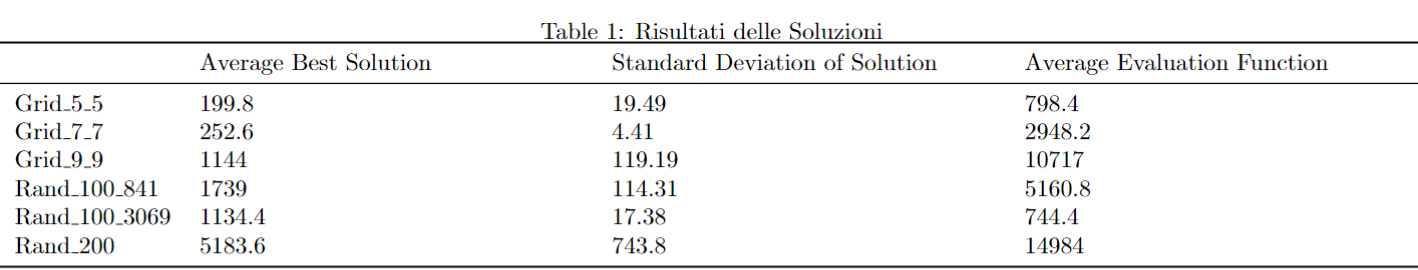
\includegraphics[width=\textwidth]{Screenshot 2025-03-03 120701.png} 
    \vspace{2pt} 
    \caption{Risultati completi relativi a tutte le istanze }
    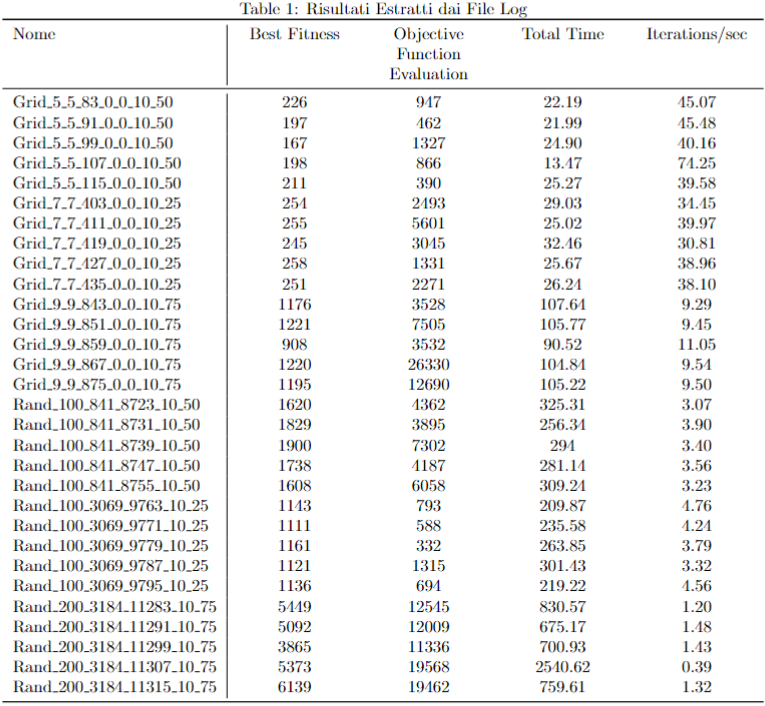
\includegraphics[width=\textwidth]{Screenshot 2025-03-03 124139.png} 
\end{figure}
L’analisi dei risultati mostra che l’hga produce soluzioni di buona qualità, stabili e con tempi di calcolo ragionevoli. Le istanze “Grid” hanno valori di fitness medi e deviazioni standard più contenuti, a conferma di una struttura più regolare, mentre le “Rand” presentano complessità maggiori, con fitness più elevati e deviazioni standard leggermente superiori. I log evidenziano un buon bilanciamento tra tempo di esecuzione e numero di iterazioni al secondo, indice di efficienza dell’implementazione. Infine, il confronto con i valori target forniti confermano che i risultati ottenuti sono validi e competitivi.
Inoltre nella maggior parte dei casi, l’algoritmo raggiunge la convergenza dopo poche centinaia di generazioni e, spesso, già entro le prime 100 ( si osservino i log nella repository presso la cartella results ). Ciò suggerisce che la creazione di una popolazione iniziale “pulita” e valida, resa possibile dal metodo di “repair”, fornisca una base di partenza solida, consentendo all’hga di trovare rapidamente soluzioni di buona qualità.
\section{Conclusioni}
Questo progetto è stata un'importante occasione di apprendimento e sperimentazione nell'affrontare il problema WFVS. Scegliere e implementare personalmente l'algoritmo HGA mi ha permesso di esaminare a fondo le dinamiche del problema, mettendo in luce il delicato compromesso tra precisione e ottimizzazione del codice. È stato particolarmente interessante osservare come, pur mantenendo risultati di alta qualità, fosse necessario analizzare attentamente le parti più onerose del codice per identificare possibili interventi di alleggerimento senza compromettere l'accuratezza. Questo approccio sperimentale e iterativo ha evidenziato la robustezza dell'algoritmo adottato, sottolineando l'importanza di bilanciare efficienza e precisione, aspetti fondamentali per risolvere con successo problemi complessi come il WFVS. In definitiva, l'esperienza ha arricchito la mia comprensione delle metodologie algoritmiche e mi ha fornito preziosi spunti per futuri miglioramenti e sviluppi.
\section{Riferimenti}
\begin{enumerate}

    \item[{[1]}] \label{2} \href{https://en.wikipedia.org/wiki/Genetic_algorithm}{Genetic algorithm}
    \item[{[2]}] \label{3} \href{https://github.com/Peppe-dmi/AI-project.git}{IA-Project, Giuseppe Nobile}
\end{enumerate}
\printindex
\end{document}